\chapter{Realizzazione di skills}
\label{chap:skills}
Mycroft permette di espandere le abilità del bot in maniera semplice: è infatti costruito modularmente, ed è in ogni momento possibile espandere o ridurre i moduli attivi.
Questi moduli sono detti \textbf{skills}. Ogni skill è responsabile di una funzionalità: avremo ad esempio la skill del meteo, la skill che racconta barzellette o la skill che si occupa della domotica. Alla ricezione di una richiesta, Mycroft verifica gli intent e le keywords di ogni skill, attivando quella giusta.
% TODO: flowchart con adapt+padatious
La creazione di nuove skills è possibile grazie alla classe Python \texttt{MycroftSkill}, tramite la cui espansione possiamo definire i comportamenti della skill. All'installazione di Mycroft verrà reso disponibile il \textbf{Mycroft Skills Kit}, una command line interface che permette di eseguire le operazioni fondamentali collegate alle skills Mycroft. Tramite il comando \texttt{mycroft-msk create} verrà avviata una CLI che, dopo aver richiesto al programmatore alcune informazioni, genera il \textit{boilerplate code} necessario alla realizzazione della skill. Tra le informazioni richieste avremo nome, frasi d'esempio, dialoghi di risposta, descrizioni, etc\dots
Il template viene inoltre fornito di \texttt{git}, un sistema di versioning che permette di tenere traccia delle modifiche al codice e semplificare l'interazione tra programmatori.
\section{Struttura dei file della skill}
La struttura delle skills è ben organizzata, e vi sono diverse tipologie di file. Oltre a licenza e README, abbiamo tre componenti fondamentali per il funzionamento.
% TODO: dirtree
\paragraph{Directory \texttt{locale}}
Questa directory contiene i file dipendenti dalla lingua. Le sottocartelle seguono i tag linguistici IETF, quindi l'italiano sarà rappresentato da \texttt{it-it} e l'inglese (americano) da \texttt{en-us}. All'interno di queste, possiamo incontrare quattro tipologie di file:
\begin{itemize}
    \item \textbf{\texttt{dialog}}: questi file contengono i dialoghi di risposta del bot. Sono presenti più frasi simili, in modo da avere interazioni più "umane" con il bot, che sceglie una frase casuale tra queste. Ad esempio, \texttt{get\_age.dialog} conterrà le frasi \textit{"Mi potresti dire quanti anni hai?"}, \textit{"Per favore, dimmi la tua età"}, \textit{"Qual è la tua età?"}...
    \item \textbf{\texttt{intent}}: questi file contengono le frasi utilizzate per addestrare la rete neurale di Padatious. Ovviamente, più esempi vengono fatti, meglio la rete funzionerà. Per esempio, il file \texttt{symptoms.bleeding.intent} conterrà frasi come \textit{"Ho un'emorragia"}, \textit{"Sto sanguinando molto"}, \textit{"Ho una grande perdita di sangue"}...
    \item \textbf{\texttt{voc}}: questi file contengono keywords utilizzate in Adapt e nelle domande a risposta chiusa. Siccome il progetto si basa fortemente su Padatious, troviamo solo i file vocabolario per le domande sì/no ed il riconoscimento di numeri. Ad esempio, il file \texttt{yes.voc} conterrà \textit{"Sì"}, \textit{"Certo"}, \textit{"Esatto"}...
    \item \textbf{\texttt{entity}}: questi file contengono entità da estrarre negli intent. Ad esempio, l'intent \textit{fratture} estrae l'arto coinvolto nella frattura. Il file \texttt{limb.entity} conterrà quindi termini come \textit{"gamba"}, \textit{"pollice"}, \textit{"spalla"}...
\end{itemize}
\paragraph{\texttt{settingsmeta.yaml}}
Questo file contiene la definizione di impostazioni modificabili dall'utente sul sito di gestione di Mycroft. Ad esempio, l'utente potrebbe voler impostare i comportamenti di default, il nome del file esportato dal bot, una chiave API per l'integrazione con altri tool.
\paragraph{\texttt{\_\_init\_\_.py}}
Questo è il file principale della skill. Contiene il codice che definisce i comportamenti della skill. Il funzionamento è basato sull'espansione della classe \texttt{MycroftSkill}, che contiene i decorator ed i metodi necessari alla gestione della skill. Il prossimo capitolo si occuperà di definire la realizzazione vera e propria.
\section{Funzionamento della skill}
Tutta la realizzazione della skill è articolata intorno alla classe \texttt{MycroftSkill}.
\begin{minted}{python}
"""Mycroft skill that does a pre-triage on hospital patients.

The skill tries to ask the patient its symptoms, its personal data, 
and more. Then, it assigns a color code, stating a priority for
medical interventions.
"""

from mycroft import MycroftSkill, intent_file_handler
import json

class HospitalTriage(MycroftSkill):
    """Main skill class for the triage.

    This is the main skill class (extending MycroftSkill),
    which contains all the operations we need to perform the
    triage.

    Attributes:
        med_record: a dict containing all the patient data.
    """

    def __init__(self):
        MycroftSkill.__init__(self)
        self.med_record = {}
\end{minted}
\subsection{Metodi relativi alle sintomatologie}
La skill è stata strutturata come segue: ogni tipologia di sintomi equivale ad un intent, ed è quindi gestita da un metodo specifico. In base alla tipologia di sintomo, l'interazione viene poi gestita in modalità diverse: verrà assegnato al paziente un codice di triage, viene confermata al paziente la corretta comprensione del sintomo, viene mostrata sulla GUI l'informazione recepita. Terminate le operazioni specifiche del sintomo, le restanti procedure vengono gestite da decorators: la richiesta dell'anagrafica, dei sintomi minori, della febbre vengono eseguite indipendentemente dal problema riportato dal paziente. Un esempio di metodo relativo alle sintomatologie può essere il seguente:
\begin{minted}{python}
# BREATH
@intent_file_handler('symptoms.breath.intent')
@symptom_handler
@covid_symptom
def handle_breathing(self, message):
    """This function handles a "breathing fatigue" symptom.

    Breathing fatigue is recognized as a red code, and is a
    COVID-compatible symptom.

    Args:
        message: the message object returned from Mycroft

    GUI: show open mouth emoji
    """
    self.gui.show_text("[emoji rimossa per motivi di stampa]")
    self.med_record["main_symptom"] = "breathing"
    self.med_record["code"] = "red"
    self.speak_dialog('symptoms.breath')
\end{minted}
Il metodo salva nell'oggetto \texttt{med\_record} (\textit{scheda clinica}) il sintomo principale, ossia problemi di respirazione, ed il codice relativo, in questo caso il rosso (accesso immediato alle cure). Poi, tramite il metodo \texttt{speak\_dialog} di \texttt{MycroftSkill}, pronuncia uno a caso tra i dialoghi contenuti nel file \texttt{symptoms.breath.dialog}, come
\begin{itemize}
    \item \textit{"Capisco, qualche problema di respirazione."}
    \item \textit{"Ok, segno nella scheda problemi di respirazione."}
    \item \textit{"Capito: problemi di respirazione."}
\end{itemize}
Da qui in poi, le operazioni sono affidate ai metodi chiamati dai decorators.
\subsection{Decorators utilizzati}
\subsubsection{Che cos'è un decorator?}
Anzitutto, occorre definire il comportamento di un decorator. Esso permette di assegnare responsabilità addizionali ad un oggetto, dinamicamente. Fornisce quindi un'alternativa flessibile al \textit{subclassing}. Definire un decorator in Python significa definire dei comportamenti da eseguire prima e dopo l'esecuzione del metodo vero e proprio.
\subsubsection{Applicazione del concetto al programma}
Alcune operazioni sono, all'interno del progetto, ricorrenti. Ad esempio, la richiesta di anagrafica o di sintomi minori deve essere fatta in tutti e soli i metodi relativi alla gestione di sintomi. Alcuni di questi (quelli compatibili con il COVID19, come la tosse), avranno bisogno inoltre di approfondimenti per valutare la possibilità che il paziente sia affetto da COVID19, facendogli domande specifiche. Sono stati quindi definiti due decorators aggiuntivi:
\paragraph{\texttt{symptom\_handler}} Questo metodo, dopo aver gestito le operazioni specifiche di un sintomo, prosegue con le procedure generali, come la richiesta dell'anagrafica, di una valutazione del dolore, di altri sintomi, e, per ultima, l'esportazione della cartella clinica.
\begin{minted}{python}
def symptom_handler(handler):
"""Decorates a symptom with the needed operations.

This function is used as a decorator for symptoms, adding
operations like personal data asking, age, other symptoms...

Returns:
    The decorator function
"""
def ask_about_symptoms(*args, **kwargs):
    returned = handler(*args, **kwargs)
    args[0].med_record["symptom_declaration"] = args[1].data["utterance"]
    # I'm using args[0] here instead of self, but it works the same
    args[0].request_age()
    args[0].request_other_symptoms()
    args[0].evaluate_pain()
    args[0].request_name()
    args[0].export_med_record()
    return returned
return ask_about_symptoms
\end{minted}
\paragraph{\texttt{covid\_symptom}} La situazione di emergenza che il mondo sta vivendo al momento della stesura di questa tesi ha richiesto particolare attenzione verso le sintomatologie compatibili con COVID19: distanziare i pazienti che potrebbero essere portatori di virus al più presto è la \textbf{sfida più grande del momento}. Per questo, il decorator, aggiunto ai soli sintomi compatibili con la malattia, permette di interrogare il paziente riguardo alcune caratteristiche tipiche della malattia, come il fiato corto, la difficoltà a percepire i sapori, la febbre alta.
\begin{minted}{python}
def covid_symptom(handler):
        """Decorates a COVID-compatible symptom.

        This function is used as a decorator in the COVID-compatible
        symptoms. It proceeds to ask the COVID-related questions
        to the patient.

        Returns:
            The decorator function
        """
        def check_if_covid(*args, **kwargs):
            returned = handler(*args, **kwargs)
            args[0].ask_covid_questions()
            return returned
        return check_if_covid
\end{minted}
Il metodo \texttt{ask\_covid\_questions} procede ad intervistare il paziente con il modello di diagnosi più usato al momento. Ogni domanda posta al paziente ha un suo \textit{score} caratteristico, che moltiplica un indice relativo al paziente in base alla gravità ed alla connessione con la malattia. Le caratteristiche indagate sono:
\begin{itemize}
    \item \textbf{Febbre}: moltiplicatore $2$
    \item \textbf{Mal di gola}: moltiplicatore $1.3$
    \item \textbf{Raffreddore}: moltiplicatore $1.3$
    \item \textbf{Fatica respiratoria}: moltiplicatore $1.6$
    \item \textbf{Tosse}: moltiplicatore $1.6$
    \item \textbf{Contatti con infetti}: moltiplicatore $2$
    \item \textbf{Mancanza di gusto}: moltiplicatore $1.7$
\end{itemize}
Ogni paziente sospetto ha inizialmente un \texttt{covid\_score} di $1$, che viene moltiplicato per i vari indici se il paziente risponde in modo affermativo. Se lo score supera una soglia predeterminata (al momento fissata a $15$), è sospetto COVID19 e verrà destinato ad un'area di triage apposita.
\begin{minted}{python}
def ask_covid_questions(self):
    """Checks for COVID symptoms.

    When triggered by a COVID-compatible symptom, 
    this function evaluates the patient symptoms to 
    try to guess if he/she has COVID19.

    GUI: show face mask emoji
    """
    self.speak_dialog('gotta_check_covid')
    covid_score = 1
    # Let's check if the patient knows the temperature. Skip if he already declared it.
    if not "fever" in self.med_record:
        self.check_fever()
    if "fever" in self.med_record:
        if self.med_record["fever"] > 37.5:
            covid_score = covid_score * 2
    # Let's define an array of tuples, each containing the yes/no question
    # string and its COVID index multiplier
    yesno_questions = [("has_sore_throat", 1.3), ("has_cold", 1.3),
     ("has_breathing_difficulties",1.6), ("has_cough", 1.6),
     ("has_had_contacts", 2), ("misses_taste", 1.7)]
    self.speak_dialog('will_ask_yesno')
    # Check if he/she has COVID-compatible symptoms
    for question in yesno_questions:
        self.med_record[question[0]] = self.ask_yesno(question[0])
        if self.med_record[question[0]] == 'yes':
            covid_score = covid_score * question[1]
        self.log.info(covid_score)

    self.med_record["covid_score"] = covid_score
    if covid_score > 15:
        self.speak_dialog('probably_has_covid')
    else:
        self.speak_dialog('doesnt_have_covid')
    self.log.info(self.med_record)
\end{minted}
\subsection{Helper methods}
Sono, oltre ai metodi caratteristici della classe, presenti alcuni \textit{helper methods} utili ad operazioni interne del software. Di seguito elenchiamo i più importanti:
\paragraph{\texttt{extract\_temperature}} Questo metodo, data una stringa in ingresso rappresentante la temperatura corporea che può essere in vari formati (ad esempio, il paziente potrebbe pronunciare \textit{"Trentasette e mezzo", "Trentasette virgola cinque", "Trentasette punto cinque", "Trentasette e cinque"} indicando sempre la stessa temperatura), la estrae in formato decimale.
\begin{minted}{python}
def extract_temperature(utterance):
    """Extracts the patient temperature from the utterance.

    This is needed because of the various ways of Mycroft interpreting
    floating point numbers. Some examples:
    - 38 e 1
    - 38/1
    - 38.1
    - 38,1
    - 38 1

    Returns:
        The floating point value of the temperature, or
        None if it is impossible to extract.
    """
    # Beware: the ' e ' has to be before the simple space!
    possible_separators = ['/', '.', ',', ' e ', ' ']
    try:
        for separator in possible_separators:
            if separator in utterance:
                temperature_strings = utterance.split(separator)
                if temperature_strings[1] == "mezzo":
                    temperature_strings[1] = "5"
                temperature = int(
                    temperature_strings[0])+float(temperature_strings[1])*0.1
                return temperature
        return None
    except TypeError:
        return None
\end{minted}
\paragraph{\texttt{age\_validator}} Questo metodo, fornito al metodo \texttt{get\_response}, definisce se un'età è valida. In caso negativo, viene chiesta nuovamente.
\paragraph{\texttt{number\_validator}} Questo metodo verifica se l'input vocale è numerico, distinguendo anche il caso in cui un \textit{sei} venga interpretato come \textit{verbo essere} e non $6$.
\subsection{Oggetto \texttt{med\_record}}
Tutti i dati della procedura di triage confluiscono in un oggetto \texttt{med\_record}, in cui vengono salvati per l'inserimento nel database ospedaliero. Questo oggetto verrà poi esportato in formato JSON (\textbf{J}ava\textbf{S}cript \textbf{O}bject \textbf{N}otation) con la possibilità di essere inviato ad un'API REST del sistema esistente.
\begin{minted}{python}
def export_med_record(self):
"""Exports the data to JSON.

This function is called at the end of the interaction
to export the fetched data from the patient. It then
assigns a desk to the patient based on his/her severeness.

GUI: show hands emoji
"""
with open("med_record.json", "w") as med_record_file:
    med_record_file.write(json.dumps(self.med_record))
self.speak_dialog('thanks_and_bye', {"desk": self.med_record["code"]})
self.med_record = {}
\end{minted}
Questo formato standard permette di essere integrato semplicemente con infrastrutture preesistenti. Per esempio, un paziente affetto da COVID19 potrebbe avere la seguente scheda clinica:
\inputminted{json}{code/med_record.json}
\section{Esempio di conversazione}
Riportiamo ora un esempio di conversazione realmente avvenuto. La conversazione è ascoltabile nei video disponibili sulla repo GitHub\cite{media:videos}.
\begin{itemize}
    \item \textbf{Utente:} \textit{Puoi aiutarmi?}
    \item \textbf{Bot:} \textit{Prima di tutto, è lei ad avere bisogno?}
    \item \textbf{Utente:} \textit{Esatto}
    \item \textbf{Bot:} \textit{Qual è il sintomo principale?}
    \item \textbf{Utente:} \textit{Ho la febbre}
    \item \textbf{Bot:} \textit{Hai la febbre, quindi. Ti sei misurato di recente?}
    \item \textbf{Utente:} \textit{Sì}
    \item \textbf{Bot:} \textit{Per favore, dimmi a quanto hai la febbre}
    \item \textbf{Utente:} \textit{Trentasette e otto}
    \item \textbf{Bot:} \textit{Mi serve qualche informazione aggiuntiva per la diagnosi. Ora ti farò alcune domande a cui rispondere sì o no. Hai male alla gola?}
    \item \textbf{Utente:} \textit{Sì}
    \item \textbf{Bot:} \textit{Soffri di raffreddore?}
    \item \textbf{Utente:} \textit{Sì}
    \item \textbf{Bot:} \textit{Noti un affaticamento quando respiri?}
    \item \textbf{Utente:} \textit{No}
    \item \textbf{Bot:} \textit{Hai la tosse?}
    \item \textbf{Utente:} \textit{Sì}
    \item \textbf{Bot:} \textit{Sei stato a stretto contatto con persone affette dal nuovo Coronavirus?}
    \item \textbf{Utente:} \textit{Sì}
    \item \textbf{Bot:} \textit{Fai fatica a sentire i sapori e gli odori?}
    \item \textbf{Utente:} \textit{Sì}
    \item \textbf{Bot:} \textit{Stiamo chiamando un medico. È possibile che tu sia affetto da COVID19. Mi potresti dire quanti anni hai?}
    \item \textbf{Utente:} \textit{Ventidue}
    \item \textbf{Bot:} \textit{Se hai altri sintomi da segnalare, dimmeli ora}
    \item \textbf{Utente:} \textit{Nient'altro}
    \item \textbf{Bot:} \textit{Come definirebbe il suo dolore da 1 a 10?}
    \item \textbf{Utente:} \textit{Sette}
    \item \textbf{Bot:} \textit{Potresti dirmi il tuo nome completo?}
    \item \textbf{Utente:} \textit{Simone Montali}
    \item \textbf{Bot:} \textit{Il tuo nome è Simone Montali, giusto?}
    \item \textbf{Utente:} \textit{Esatto}
    \item \textbf{Bot:} \textit{Grazie per la pazienza, recati al banco YELLOW}
\end{itemize}
\begin{figure}[h]
    \begin{center}
        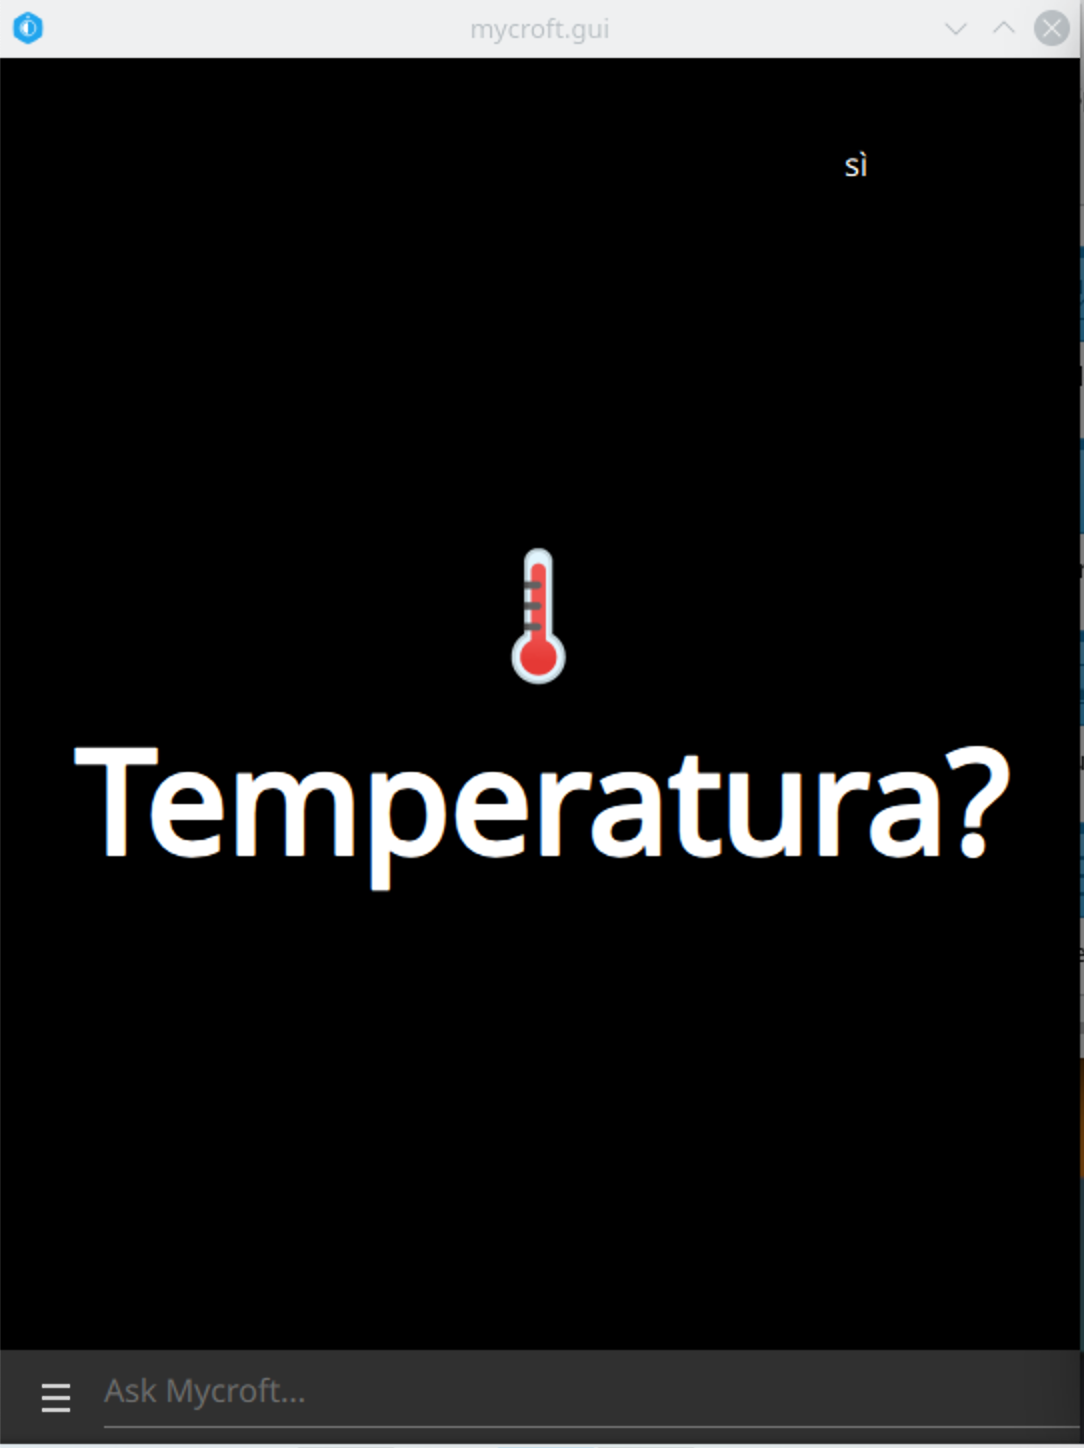
\includegraphics[width=0.45\columnwidth]{images/skills/temperature.png}
        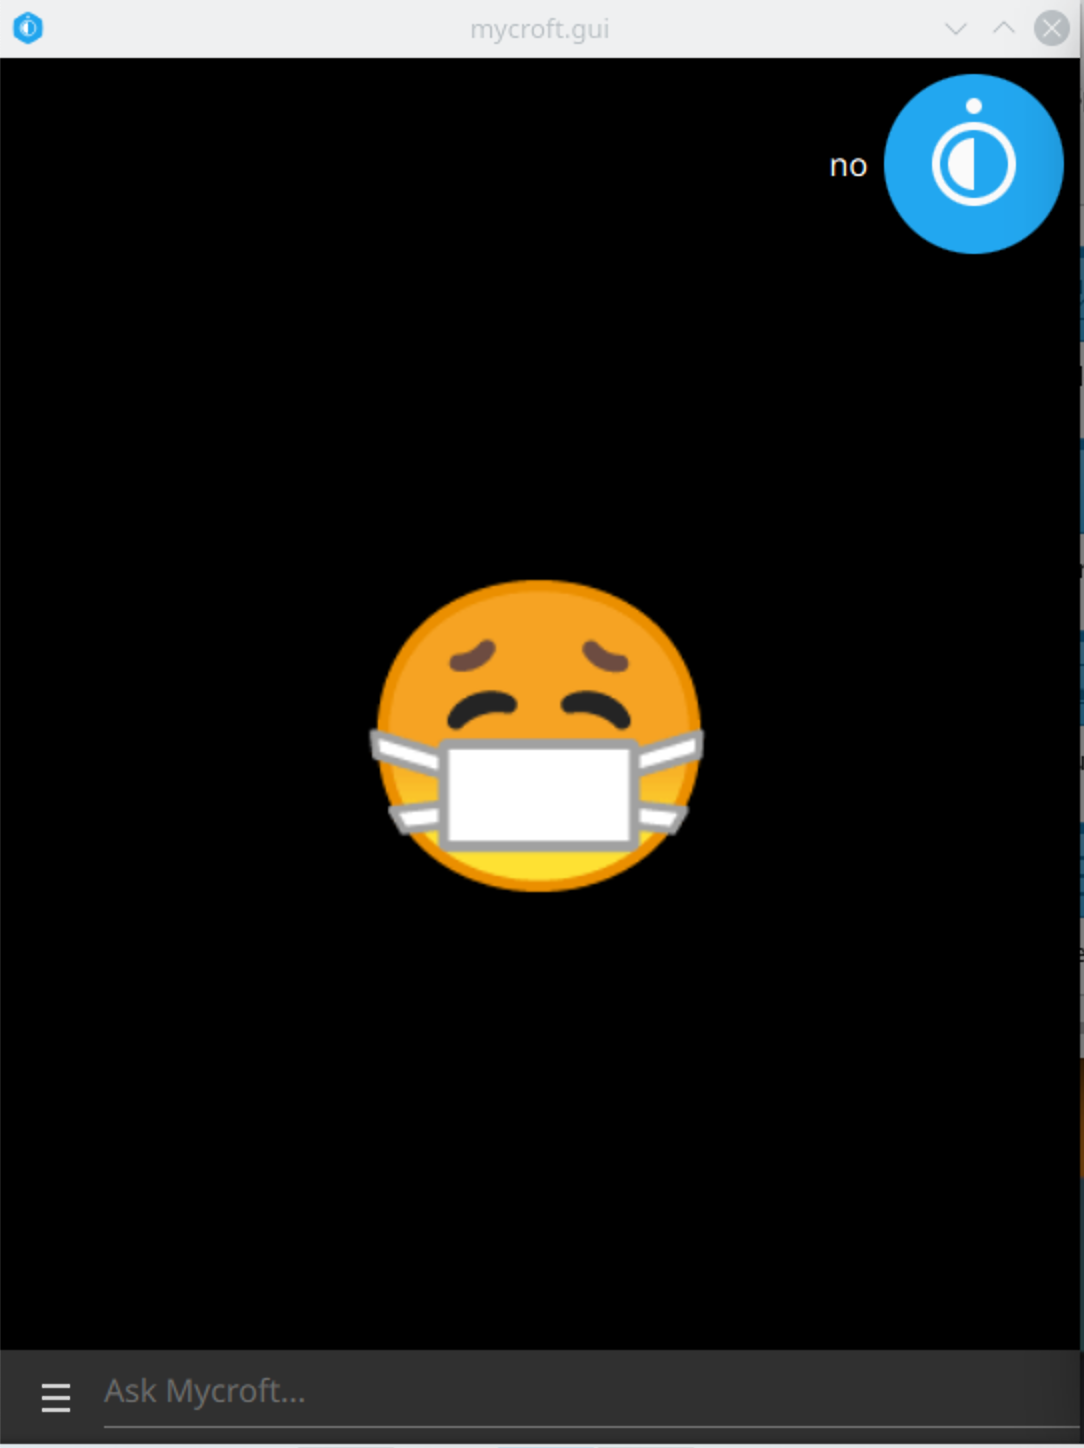
\includegraphics[width=0.45\columnwidth]{images/skills/facemask.png}
    \end{center}
    \caption{Alcune schermate della GUI durante la diagnostica del COVID19}
    \label{fig:gui-screens}
\end{figure}